%\RequirePackage[l2tabu, orthodox]{nag}  %Checks for older packages 

\documentclass[11pt,a4paper]{article}
% \documentclass[10pt]{extreport} $ allos to make the font smaller
\usepackage[utf8]{inputenc}

\usepackage{amsmath}
\usepackage{amsfonts}
\usepackage{indentfirst}
\usepackage{amssymb}
\usepackage{siunitx}  % Units of the metric system  \SI{2.63}{\ohm}   
\usepackage[font={footnotesize}]{caption} %Makes the captions small

\usepackage{algorithm}
\usepackage{algpseudocode}

%% Figures packages
\usepackage[pdftex]{graphicx}
\usepackage{float}   %Es para colocar el objeto flotante exactamente donde se ponga el comando con H
\usepackage{caption}
\usepackage{subcaption}
\graphicspath{{../results/}}
\usepackage{sidecap}  %Para poner figuras a los lados


\usepackage{setspace} % Needed for Pyton syntax highlight
\usepackage{listings}    % Include the listings-package, nice verbatim for code
\usepackage{color}
\usepackage{courier}


\usepackage{cleveref} %puts figure and equation appropiately \cref{} 

\usepackage{natbib} %For bibliography
%\usepackage{cite}
\usepackage{framed} % To use boxes, or frames around text

\usepackage{parskip} %Para saltos entre parrafos
\setlength{\parindent}{0pt} 
\setlength{\parskip}{\baselineskip}
\usepackage[a4paper,margin=0.8in]{geometry}  %%Cambiar los margenes

\newcommand{\HRule}{\rule{\linewidth}{0.5mm}}

%\usepackage{hyperref} %This should be loade after most of the other packages 
% \hypersetup{colorlinks=true}  %Para que los hiperlinks cuando se hagan referencias aparezcan en colores.

% This is for the Python Package
\definecolor{Code}{rgb}{0,0,0}
\definecolor{Decorators}{rgb}{0.5,0.5,0.5}
\definecolor{Numbers}{rgb}{0.5,0,0}
\definecolor{MatchingBrackets}{rgb}{0.25,0.5,0.5}
\definecolor{Keywords}{rgb}{0,0,1}
\definecolor{self}{rgb}{0,0,0}
\definecolor{Strings}{rgb}{0,0.63,0}
\definecolor{Comments}{rgb}{0,0.63,1}
\definecolor{Backquotes}{rgb}{0,0,0}
\definecolor{Classname}{rgb}{0,0,0}
\definecolor{FunctionName}{rgb}{0,0,0}
\definecolor{Operators}{rgb}{0,0,0}
\definecolor{Background}{rgb}{0.98,0.98,0.98}

\lstnewenvironment{python}[1][]{
\lstset{
numbers=left,
numberstyle=\footnotesize,
numbersep=1em,
xleftmargin=1em,
framextopmargin=2em,
framexbottommargin=2em,
showspaces=false,
showtabs=false,
showstringspaces=false,
frame=l,
tabsize=4,
% Basic
basicstyle=\ttfamily\small\setstretch{1},
backgroundcolor=\color{Background},
language=Python,
% Comments
commentstyle=\color{Comments}\slshape,
% Strings
stringstyle=\color{Strings},
morecomment=[s][\color{Strings}]{"""}{"""},
morecomment=[s][\color{Strings}]{'''}{'''},
% keywords
morekeywords={import,from,class,def,for,while,if,is,in,elif,else,not,and,or,print,break,continue,return,True,False,None,access,as,,del,except,exec,finally,global,import,lambda,pass,print,raise,try,assert},
keywordstyle={\color{Keywords}\bfseries},
% additional keywords
morekeywords={[2]@invariant},
keywordstyle={[2]\color{Decorators}\slshape},
emph={self},
emphstyle={\color{self}\slshape},
%
}}{}



\definecolor{dkgreen}{rgb}{0,0.6,0}

\title{Lab12: DD2380 }
\author{
Ramon Heberto Martinez Mayorquin  hramon@kth.se 
Akash Kumar Dhaka  akashd@kth.se 
}



\begin{document}

\begin{titlepage}
\begin{center}
%\includegraphics[width=0.15\textwidth]{logo}\\[1cm]    

\textsc{\LARGE Kungliga Tekniska högskolan}\\[1.0cm]

\textsc{\Large Class: DD2432 Artificial Neural Networks}\\[2.0cm]



\begin{figure}[H]
	\centering
 
\includegraphics[width=0.35\textwidth]{Kth_logo.png}
\end{figure}
%\\[1cm]    


% Title
\HRule \\[0.4cm]
{ \huge  Project: Deep Neural Networks in Theano
}\\[0.4cm]
\HRule \\[1.5cm]

% Author and supervisor

Author: Ram\'on Heberto Mart\'inez \\ 
\large Professors: Erik Frans\'en, Pawel Herman  \\ [2.5cm]
%\normalsize Presenta \\
%\large Supervisors 2: Jan Antolik \\[2.5cm]

\textsc{\Large School of Computer Science and Communication }\\ [1.0cm] 
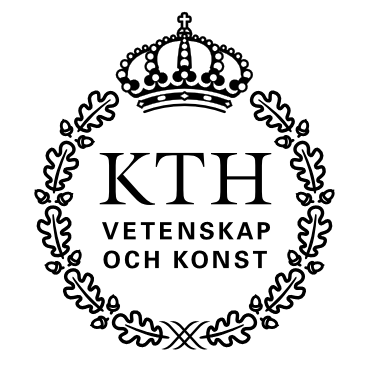
\includegraphics[width=0.15\textwidth]{KTH_black.png}\\[1.5cm] % Controls the distance till the new object 
% Bottom of the page
{\large 31 May of 2015}

\end{center}
\end{titlepage}

%%%%%%%%%%%%%%%%%%%%%%%%%%%%%%%%%%%%
%%%%%%%%%%%%%%%%%%%%%%%%%%%%%%%%%%%%
% Abstract
%%%%%%%%%%%%%%%%%%%%%%%%%%%%%%%%%%%%
%%%%%%%%%%%%%%%%%%%%%%%%%%%%%%%%%%%%
\begin{abstract}
In this work we have explored some basic deep architectures with the Theano library. We worked with an implementation of the Multilayer Perceptron, The Restricted Boltzmann Machine and Deep Belief Networks and explored their functionality and capabilities. We present here a discussion of of the advantages and disadvantages of those approaches implemented with the mentioned library and also the different results of those investigations.
\end{abstract}

%%%%%%%%%%%%%%%%%%%%%%%%%%%%%%%%%%%%
%%%%%%%%%%%%%%%%%%%%%%%%%%%%%%%%%%%%
\section{Introduction}
%%%%%%%%%%%%%%%%%%%%%%%%%%%%%%%%%%%%
%%%%%%%%%%%%%%%%%%%%%%%%%%%%%%%%%%%%

In this section we present the two technical components of our work. First we speak about the data set that we use to work and understand the techniques of deep learning and we also talk about the library that we use to implement the required algorithms. 

%%%%%%%%%%%%%%%%%%%%%%%%%%%%%%%%%%%%
\subsection{The MNIST Data Set}
The \textbf{MNIST}  data set (\cite{lecun1998mnist}) is a set of images used widely in the field of Machine Learning in general and Visual Recognition in particular. The set consists of hand-written digits from different people. We show a sample of the images in figure \ref{fig:mnist_example} were we can appreciate the variability inter digit and among the digits. 

%% Figure %% 
\begin{center}
\begin{figure}[H]
\centering
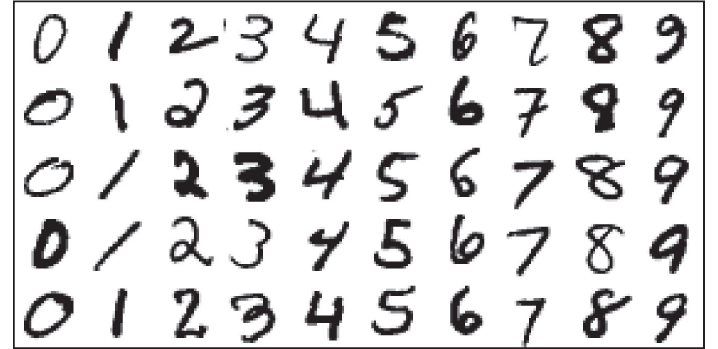
\includegraphics[scale=.45]{mnist_example.png} 
\caption{A sample from the MNIST dat set. In total it possess $60000$ training samples and $10000$ images.  We can see that we have both variability within the digits and among the digits..}
\label{fig:mnist_example}
\end{figure} 
\end{center}

The set was formed by combining two data sets of the National Institute of Standars and Technology (NIST) from the United States. One of them consisted on hand 
-written digits by high school students and the other is composed of the same elements but written by employees of the United States Census Bureau. 

%%%%%%%%%%%%%%%%%%%%%%%%%%%%%%%%%%%%
\subsection{Theano}
\textbf{Theano} is a python library that implements symbolic differentiation and evaluation of expressions involving arrays of multiple dimensions (\cite{bergstra2010theano}). The library was developed in the research environment of the University of Montreal and is extensively used in the Deep Learning community as a library that is powerful, efficient and provides ample room for experimentation. 

In this work we will be implementing the algorithms in \textbf{Theano}. Along this work we will mentioned how the capabilities of Theano allow us to carry the task at hand in an easy an convenient way. 

%%%%%%%%%%%%%%%%%%%%%%%%%%%%%%%%%%%%
%%%%%%%%%%%%%%%%%%%%%%%%%%%%%%%%%%%%
\section{Algorithms}
%%%%%%%%%%%%%%%%%%%%%%%%%%%%%%%%%%%%
%%%%%%%%%%%%%%%%%%%%%%%%%%%%%%%%%%%%

In total we implemented three algorithms using the templates that the \textbf{Theano} library provides: the Multilayer Perceptron, a Restricted Boltzmann machine trained by constrastive divergence and a Deep Belief Network. In this section we briefly describe their architecture and how they fit within the architectural constrains of Theano.

%%%%%%%%%%%%%%%%%%%%%%%%%%%%%%%%%%%%
\subsection{Multilayer Perceptron}

The Multilayer perceptron is an artificial neural network without recurrent connections (that is feedfoward) that is a generalization of the linear perceptron. Its strength is that it can distinguish data that is not separable. We present the archicture of our network in figure \ref{fig:mlp}. 

\begin{SCfigure}[][h]
  \centering
  \caption{Here we describe the architecture of the Multilayer Perceptron. In the left side of the picture we have the inputs, as inputs the neuron receives the raw data that we are interested in classifying (or using regression), we call the input side the input layer. The input layer should have as many units as dimensions has the data that we are interested in classifying. The layer in between is called the hidden layer and is the responsible or building another representation of our data where the non-linear data is separable. Finally the output layer in the right reveals with its activation to which category the input belongs (or provides the value if it is regression).  }
  \includegraphics[width=0.4\textwidth]%
    {MLP.jpg}% picture filename
	\label{fig:mlp}
\end{SCfigure}


The architecture can be represented mathematically by the following formula

\begin{align*}
f(x) = G(b^2 + W^2 (\underset{Hidden Layer}{s(b^2 + W^1x)}))
\end{align*}

The Hidden layer is built by multiplying the first matrix of coefficients, adding the bias and then a non-linear transformation $s$ to produce the hidden layer as indicated with text in the equation above. After that the Hidden layer is then transformed again by the same process to obtain the input. The superscript in the equation indicates the level of deep that the layer belongs too and is not a power in the mathematical sense. 

Now, let's suppose that we have a data set $D$ composed of inputs $x_i$ and outputs $y_i$. In order to train the algorithm we need to define a \textbf{loss function} that will let us know in which direction we have to move our parameters so our output is better predicted given the model. For the MLP we define the loss function through the likelihood function:

\begin{align*}
\mathcal{L}(\theta = \{W, b\}, D) = \sum_{i=0}^{D} 
\log(P(Y = y^i | x^i , W, b	))
\end{align*}

Where the probability $P(Y = y^i | x^i , W, b	)$ can be defined as a \textbf{softmax function} in the last layer. The prediction consequently is the output layer for which the probability is maximal.  With this in our hands we can converge to our parameters by moving in the direction that minimizes the negative of the likelihood above. The usual way to achieve this is through the \textbf{Backpropagation Algorithm} that allow us to calculate the gradient of the error with respect to all parameters but with the symbolic capabilities of \textbf{Thean} this can be done using only the following lines of code:


\begin{python}
g_W = T.grad(cost=cost, wrt=classifier.W)
g_b = T.grad(cost=cost, wrt=classifier.b)
\end{python}

Where the classifier is just the class instatiation of our algorithm and cost is the negative of the function presented above. After this the update rules is written as a simple as:

\begin{center}
\begin{python}
updates = [(classifier.W, classifier.W - learning_rate * g_W),
           (classifier.b, classifier.b - learning_rate * g_b)]
\end{python}
\end{center}

With both this expressions we can use a function that updates the parameters at every training step and as simple as that Theano performs a step of gradient descent. 

%%%%%%%%%%%%%%%%%%%%%%%%%%%%%%%%%%%%
\subsection{Restricted Boltzmann Machine}

A Restricted Boltzmann Machine is a neural network that has hidden layer and can learn the distribution over the observable layer. They were discovered at the end of the eighties by Paul Smolensky and called Harmonium back then (\cite{mcclelland1986parallel} Chapter 6) but the training algorithms were slow. It was not until the middle of the last decade that fast algorithms to train them were discovered (\cite{hinton2006reducing}). We present a graphical representations of their architecture in the figure \ref{fig:rbm}.


\begin{SCfigure}[][h]
  \centering
  \caption{Here we describe the architecture of the Restricted Boltzmann Machine. put belongs (or provides the value if it is regression).  The visible units are represented to the left and they correspond to the inputs, that is, they are usually the data that we have and we are interesting in modeling. In the right we have the hidden units, this is the part of the system in charge of representing features and hidden relations in our data. In opposition to complete Boltzmann Machine there are no connections within any of the layers, the only connections are between them.  }
  \includegraphics[width=0.35\textwidth]%
    {rbm.png}% picture filename
	\label{fig:rbm}
\end{SCfigure}


The Restricted Boltzman Machine is an energy model. That means that we represent the probability of a particular input in terms of an energy function in the following way:

\begin{align*}
p(v) = \frac{e^{-E(v)}}{Z}
\end{align*}

Where $Z$ is just a normalizing factor that is constructed by summing the denominator in the equation above through all the possible values of the input and makes $p$ a probability distribution. 

The idea here is to make our data the most probably with a certain energy function. In this case though, we have hidden units and we are interesting in the distribution over the observable units. So in order to get that distribution we can marginalize in the usual way:

\begin{align*}
P(v) = \sum_{h} P(v,h) = \sum_{h} \frac{e^{-E(v, h)}}{Z}
\end{align*}

Where the v represents a unit from the visible layer and h a unit from the hidden layer. Being specific in the case of the RBM's the energy function takes the following form:

\begin{align*}
E(v, h) = -bv -ch - hWv 
\end{align*}

Where $b$ and $c$ are the bias term of the visible layer and the hidden layer respectively. Finally $W$ is the matrix that encodes the connections between the layers. Is those parameters the ones that we have to adjust in order to make the system give the highest probability to the actual data that we show to it. 

Following inspiration from Physics we introduce a quantity called the \textbf{Free Energy}: 

\begin{align*}
\mathcal{F}(x) = - \log \sum_{h} e^{E(x, h)}
\end{align*}

Give the energy above the free energy then is:

\begin{align*}
\mathcal{F}(x) = -bv - \sum_i \log_{h_i} e^{h_i(c_i + W_i v)}
\end{align*}

Regarding the question of how to train this type of mode the answer is that we can, as usual, perform gradient descent on the empirical negative log-likelihood which we define as: 


\begin{align*}
\mathcal{L}(\theta, D) = \frac{1}{N} \sum_{x \in D} \log p(x)
\end{align*}

But if we come back to the free energy expression in turns out that we can represent the derivative in the sum above in the following way:

\begin{align*}
- \dfrac{\partial{\log p(x)}}{\partial{\theta}} = \dfrac{\partial{\mathcal{F}(x)}}{\partial{\theta}} - \sum_{y} p(y) \dfrac{\partial{\mathcal{F}(y)}}{\partial{\theta}}
\end{align*}

The term in the left is know as the \textbf{positive face} and ire responsible for increasing the probability of the training data. The second term, on the other hand, is called \textbf{negative phase} and its function is to reduce the probability of the data generated by the model (\cite{yoshua2009learning}).

The positive phase term is easy to compute. We only calculate the gradient of the free energy at our particular example. The second term on the hand requires an average of the gradient of the free energy over the total number of possible configurations which is in most of the cases not tractable. In order to simplify the task what we do in to use \textbf{Monte Carlo} methods. In particular we create a Markov Chain and perform Gibbs sampling to obtain samples from the underlying distribution. 

An important further step to make the training of the RBM's fast enough is the form in which we computer the Gibbs sampling. Two famous tricks are \textbf{Constrastive Divergence} (CD-k) where the first term of the chain is sampled from the training data and \textbf{Persistent CD} where the state of the chain is preserved at the end of the sampling for the next iteration. 

It is important to mention that usually we need to express the free energy as an analytically expression but with the symbolic capabilities of Theano the code allows us to actually calculate the gradient from the expression above. 

\begin{python}
   # determine gradients on RBM parameters
        # note that we only need the sample at the end of the chain
        chain_end = nv_samples[-1]

        cost = T.mean(self.free_energy(self.input)) - T.mean(
            self.free_energy(chain_end))
        # We must not compute the gradient through the gibbs sampling
        gparams = T.grad(cost, self.params, consider_constant=[chain_end])
\end{python}

Where the variable chain end was obtained from the Gibbs sampling mechanism (is the last sample of the visible layer). The mean over there is because we are using a min-batches approach to regression and therefore we move in the direction of the batch. Note that this symbolical calculation of the gradient saves us a lot of problems in the domain of numerical stability and makes the algorithm overalls cleared (although harder to implement because it requires a different type of thinking).

%%%%%%%%%%%%%%%%%%%%%%%%%%%%%%%%%%%%
\subsection{Deep Belief Networks}


Deep Belief Networks can be though of the combination of the two  algorithms that we presented above. Until the middle of the last decade most experiments with networks with more than two hidden layers initiated randomly performed poorly (\cite{bengio2009learning}). However, the breakthrough come when it was realized that the multiple layers could be trained with an unsupervised algorithm in a greedy way and then do fine tuning with supervised algorithms as usual. We show the general architecture of DBNs in \ref{fig:dbn} and describe the algorithm in more detail bellow. 


\begin{SCfigure}[][h]
  \centering
  \caption{Here we describe the architecture of the Deep Belief Network. In general we have an $n$ number of hidden layers. The first layers is the input layers and is used to train the second layer with an unsupervised method (in this case RBM). Then, once trained, the second layer is used used as an input to train the third layer in the same way and so on. At the end a supervised learning method is used for fine tuning all the parameters. (Image taken from the Lisa Lab wikipage)}
  \includegraphics[width=0.5\textwidth]%
    {dbn.png}% picture filename
	\label{fig:dbn}
\end{SCfigure}


The principle to train DBN's in a greedy wise has been described before in \citep{bengio2007greedy} here we resume it for the sake of completeness:

\begin{enumerate}
\item Train the first layer as an RBM that models the raw input data, that is $x = h_0$.
\item Use the first layer to build a representation that will be used in the second layer. A common way to do that is to use the mean activation: $p(h_1 = 1 | h_0)$.
\item Use this representation to train the second layer as the hidden layer of another RBM where the inputs are these activation values. 
\item Iterate until the last layer.
\item Fine tune all the parameters of the deep architecture with a supervise learning algorithm. 
\end{enumerate}

In this work we used RBM's for the pre-training and then we did the fine tuning with the same method that we use for the MLP above. At the level of implementation the critical part is to construct the weights and parameters as shared values that are shared both by the class of the MLP and the class of the RBM's.

\begin{python}
            # Construct an RBM that shared weights with this layer
            rbm_layer = RBM(numpy_rng=numpy_rng,
                            theano_rng=theano_rng,
                            input=layer_input,
                            n_visible=input_size,
                            n_hidden=hidden_layers_sizes[i],
                            W=sigmoid_layer.W,
                            hbias=sigmoid_layer.b)
            self.rbm_layers.append(rbm_layer)

\end{python}

Here the sigmoid layer is the layer of the MLP. What we are doing is to share the weight and bias parameters of the sigmoid layer with the RBM. Then at the end we append it to a list with all the layers. Finally, as usual the gradient with respect to all the parameters can be computed symbolically avoiding numerical problems.

\begin{python}
# compute the gradients with respect to the model parameters
        gparams = T.grad(self.finetune_cost, self.params)

\end{python}


%%%%%%%%%%%%%%%%%%%%%%%%%%%%%%%%%%%%
\section{Results}
%%%%%%%%%%%%%%%%%%%%%%%%%%%%%%%%%%%%

Here we present the result of our experiments

%%%%%%%%%%%%%%%%%%%%%%%%%%%%%%%%%%%%
\subsection{Multilayer Perceptron}



%%%%%%%%%%%%%%%%%%%%%%%%%%%%%%%%%%%%
\subsection{Restricted Boltzmann Machine}

%%%%%%%%%%%%%%%%%%%%%%%%%%%%%%%%%%%%
\subsection{Deep Belief Networks}

%%%%%%%%%%%%%%%%%%%%%%%%%%%%%%%%%%%%
\section{Discussion}
%%%%%%%%%%%%%%%%%%%%%%%%%%%%%%%%%%%%

In this work we have explored the most basic deep learning algorithms with Theano using the MNIST data set. Along these work we have emphasize how the library how the symbolic capabilities of Theano aided us to get rid of numerical stability and implementation issues by constructing gradient descent algebraically instead of implicitly. Furthermore the symbolic construction of the library allowed us to run our algorithms in the GUP without any extra effort. 

-We have done this algoriths and obtain this, this compares to so and so in the literature.

- I have learn that: 
Regarding deep learning it is clear to me now that the power of the models resides in creating sound statistical representations that gives us further information about our data, those could be called features. A very interesting parallel is in Cognitive Neuroscience were abstract models can be used to accomplish a complex task. In a further work we would like to explore more this line of thinking. 

Moreover we are also aware of the limitations of deep learning architectures. The increase in the number of layers brings a massive computational problem that can create a bottleneck in the progress of the field. Furthermore the complexity (algorithmic-wise and conceptually) of the techniques and concepts create a barrier of entry for understanding and maintaining them.

Finally there are other types of deep neural networks that were not included in this preliminary study.  For image processing Convolutional Neural Networks have been the standard on the field for quite a while. As an alternative for the unsupervised part in the DBN Denoising Auto-Encoders can be used. Furthermore there are more exotic and bedding architectures down the line like Compund Hierachial=Deep Models with a Bayesian inspiration and interpretation. It is of our interest to further explore the capabilities of neural networks to represent short and long-term temporal relationships with temporal data. A natural candidate to accomplish that role are Recurrent Neural Networks, in a further work we would like to address that particular aspect.

\bibliographystyle{plainnat}
\bibliography{ref_deep_learning}
\end{document}